
\documentclass[11pt, letterpaper]{article}
\usepackage{geometry}
\usepackage{graphicx}

\geometry{margin={1.25in, 1.25in}}

\title{An Algorithm for Obstruction-free Double-Ended Queues}
\author{Sean Brennan}
\date{May 1, 2013}

\begin{document}
    \maketitle

    \begin{abstract}
        This paper describes a nonblocking algorithm for implementing a data structure known as a double-ended queue. There have only been a handful of algorithms for nonblocking deques, each of which has deficiencies including boundedness of size, reduced concurrency, and a need for special atomic primitives. With the help of Michael Scott, I have devised a new approach built off of prior work from Herlihy et al. that achieves four highly desirable properties: \emph{unboundedness}, \emph{space efficiency}, \emph{high concurrency}, and finally \emph{obstruction-freedom}. Some preliminary analysis shows that this nonblocking double-ended queue can provide significantly higher throughput than a similar algorithm using mutual exclusion.
    \end{abstract}

    \section{Introduction}
        \subsection{Nonblocking Algorithms}
            An algorithm is described as \emph{nonblocking} if it guarantees that separate threads of execution which share some resource cannot be blocked - that is, halted indefinitely. This class of algorithms is highly desirable because they allow the programmer to forgo locks and mutual exclusion. While mutual exclusion is understandable intuitively and has been put to use in a wide range of applications, it has its flaws. Locks can easily lead to very subtle and difficult to track program bugs: deadlock, livelock, the convoy effect, and priority inversion are just a few examples. From a pragmatic standpoint, blocking on locks also wastes cycles that a thread could be using to accomplish more meaningful work.

            Despite these benefits, nonblocking algorithms carry the tradeoff of extremely complex code. Nonblocking algorithms must be written such that a thread can be halted anywhere in its execution, wake up some unknown amount of time in the future, and be able to recognize whether it should continue with its operation or try again. This makes these algorithms very difficult to write and to test. Furthermore, different flavors of nonblocking algorithms provide different levels of guarantees about their behavior that can complicate their implementations even more.

            \begin{itemize}
                \item \emph{Obstruction-free}: This class of nonblocking algorithms is the weakest. It specifies that some thread, in the absence of contention, will always complete its operation in a bounded number of steps. All this ensures is that the system is free of \emph{deadlock}.
                \item \emph{Lock-free}: This class of nonblocking algorithms builds on the guarantees of obstruction freedom. It specifies that some thread will always complete its operation in a bounded number of steps. It follows from this principle that if some thread's operation fails, it is always because some other thread's operation succeeded. This means that the system is free of \emph{deadlock} as well as \emph{livelock}.
                \item \emph{Wait-free}: This class of nonblocking algorithms is the strongest and builds on the guarantees of lock freedom. To summarize this property more succinctly, all threads in a wait-free algorithm must complete their operations in a bounded number of steps. On top of \emph{deadlock} and \emph{livelock}, wait-free algorithms remove the problem of \emph{starvation}.
            \end{itemize}

            The rest of this paper is focused solely on obstruction-free algorithms. These algorithms have the easiest properties to prove and tend to be the simplest to implement.

        \subsection{Double-Ended Queues}
            A double-ended queue, or \emph{deque}, is a very powerful and useful data structure. It builds off the notion of the classical FIFO queue, which has a tail for enqueueing items and a head for dequeueing items. The deque extends this data structure by allowing the programmer to push and pop to and from both ends of the queue. For this reason, deques are able to generalize FIFO structures (queues) and LIFO structures (stacks) easily well. Furthermore, if one has a nonblocking algorithm for deques, then one trivially has a nonblocking algorithm for stacks and queues as well.

    \section{Previous Work}
        Despite the power of the double-ended queue abstraction, there are so far only a handful of papers concerning nonblocking implementations of these structures. Each has its own strengths and weaknesses, but none so far guarantees the suite of properties that I would like to achieve with my algorithm: \emph{unboundedness}, \emph{space efficiency}, \emph{high concurrency}, and \emph{obstruction-freedom}. Each has nevertheless lent inspiration to my algorithm, even if only a small amount.

        The first paper is Michael's ``CAS-Based Lock-Free Algorithm for Shared Deques'' \cite{michael}. In this paper, Michael describes how to implement a lock-free deque. Michael's algorithm achieves this through the use of a double-wide compare-and-swap operation that updates an \emph{anchor} variable, which keeps track of references to the two queue ends. After each successful push operation, a participating thread attempts to \emph{stabilize} the structure by making sure all nodes are connected to one another; if this stabilize operation fails, then the next pop operations attempts it before continuing.

        The Michael deque is powerful, but has its share of shortcomings. In terms of strengths, it is \emph{unbounded}, which the next algorithm I will discuss is not. Furthermore, its guarantees of behavior make it \emph{lock-free}, while I propose only to implement an obstruction-free algorithm. Finally, Michael describes several simple extensions to the algorithm to make it highly \emph{space-efficient}. The biggest problem with this deque is its lack of concurrency between ends. It serializes all updates to the deque, meaning that a left pop can cause a right push to abort, for example. In the average use case, this ``interference'' is completely artificial. Furthermore, the call for a double-wide compare-and-swap could restrict the architectural possibilities of the algorithm.

        These problems are addressed in ``Obstruction-Free Synchronization: Double-Ended Queues as an Example'' by Herlihy et al \cite{herlihy}. Using the compare-and-swap primitive, they are able to create a much more concurrent deque that is also obstruction-free. Rather than use the more conventional pointer-based approach for constructing queues, the authors elect to create the queue in contiguous memory and use special null values to identify the two queue ends. I will spare a more detailed description of the algorithm, since a description of my algorithm will cover most of the details of theirs as well.

        The main strength of the Herlihy et al. deque over the Michael deque is its \emph{concurrency between ends}. Rather than serialize entire operations on the deque, the authors serialize each modification of an individual node. This means that only two concurrent operations to the same end will conflict. A simple extension that makes the deque's buffer circular also greatly increases \emph{space efficiency}. The primary weakness of this deque is that it is \emph{bounded} - it can only hold as many elements as there is space originally specified.

        One additional paper, ``Fast Concurrent Queues for x86 Processors'' by Afek and Morrison \cite{afek}, provides hope that a best-of-all-worlds deque implementation can be constructed. This paper describes a lock-free FIFO queue that is unbounded in size and and also space efficient. This is achieved through ``chunking'' the queue into discrete cyclic arrays, which are then chained together into a linked list. Michael Scott and I believe that this chunking approach can be easily ported over to the deque space as an extension of the Herlihy et al. algorithm.

    \section{The Algorithm}
        \begin{figure}[t!]
            \footnotesize\begin{verbatim}
type element = record val: valtype; ctr: int end
A: array[0..MAX+1] of element initially there is some k in [0,MAX]
    such that A[i] = <LN,0> for all i in [0,k]
    and A[i] = <RN,0> for all i in [k+1,MAX+1].

rightpush(v) // v is not RN or LN
     while (true) {
         k := oracle(right); // find index of leftmost RN
         prev := A[k-1]; // read (supposed) rightmost non-RN value
         cur := A[k]; // read (supposed) leftmost RN value
         if (prev.val != RN and cur.val = RN) { // oracle is right
             if (k = MAX+1) return "full"; // A[MAX] != RN
             if CAS(&A[k-1],prev,<prev.val,prev.ctr+1>) // try to bump up prev.ctr
                 if CAS(&A[k],cur,<v,cur.ctr+1>) // try to push new value
                     return "ok"; // it worked!
             } // end if (prev.val != RN and cur.val = RN)
         } // end while
rightpop()
     while (true) { // keep trying till return val or empty
         k := oracle(right); // find index of leftmost RN
         cur := A[k-1]; // read (supposed) value to be popped
         next := A[k]; // read (supposed) leftmost RN
         if (cur.val != RN and next.val = RN) { // oracle is right
             if (cur.val = LN and A[k-1] = cur)"; // adjacent LN and RN
                 return "empty
             if CAS(&A[k],next,<RN,next.ctr+1>) // try to bump up next.ctr
                 if CAS(&A[k-1],cur,<RN,cur.ctr+1>) // try to remove value
                     return cur.val // it worked; return removed value
             } // end if (cur.val != RN and next.val = RN)
         } // end while
            \end{verbatim}
            \caption{Pseudo-code of the original bounded deque from the Herlihy et al. paper \cite{herlihy}. Left operations are completely symmetrical with right operations.}
            \label{code::bounded}
        \end{figure}

        This algorithm builds primarily off of the Herlihy et al. implementation of a bounded double-ended queue \cite{herlihy}. (For the sake of convenience, I will henceforth refer to this as the Herlihy deque) Therefore, I will begin with a more in-depth description of that algorithm.

        \subsection{Bounded Description}
            The Herlihy deque begins with a segment of contiguous memory as large as the maximum number of elements in the deque, plus two additional boundary nodes that mark the end of the memory region. Each entry in the region constitutes a node, which has a pointer to some value and a counter which will be described later. The region is initialized so that all nodes have one of two special null values: LN and RN. The ``left half'' of the region contains the LNs, and the ``right half'' contains the RNs. An invariant of the deque that must hold over all operations follows: the deque must consist of one or more LNs, followed by zero or more non-null values, followed by one or more RNs.

            Each operation on the deque first begins with a call to an oracle function. This function returns what it believes to be the current position of either the left head or the right head. This oracle function can be implemented however one desires, as long as it 1) returns [0, SIZE - 2] and [1, SIZE - 1] for left and right operations respectively, and 2) is accurate in the absence of contention with other threads. I will discuss my own implementation of the oracle function in the next section, which uses hints to locate the heads.

            Next, a copy of the head and an adjacent element are loaded into local memory. We first check that the oracle function is correct by confirming that the following invariants hold:
            \begin{itemize}
                \item The \emph{left head} at \emph{i} must be an LN node, with the \emph{i + 1} node being non-LN.
                \item The \emph{right head} at \emph{i} must be an RN node, with the \emph{i - 1} node being non-RN.
            \end{itemize}
            If this condition is not the case, the oracle was inaccurate and we immediately retry the operation. If this condition passes, we then quickly check whether the deque is either full or empty. It is full if the head is at a boundary node; it is empty if an adjacent LN and RN are witnessed (this follows from the earlier stated deque invariant).

            Finally, each push and pop performs two compare-and-swap operations. It first examines the head's adjacent node and attempts only to modify its counter, trying again immediately if the operation fails. This is necessary to avoid the ABA problem. If this operation succeeds, it tries to either push a new element to the head position or remove some element from the adjacent position.

            Figure \ref{code::bounded} shows some example code from the original Herlihy et al. paper. Note the possibility of livelock. A thread pushing right is preempted right after its first CAS. Another thread attempts to do a right pop and is then preempted after its first CAS. The first thread wakes up, fails on its second CAS, and retries, succeeding again in its first CAS. This causes the second thread to fail its second CAS, ad infinitum.

        \subsection{Unbounded Description}
            Fortunately, this deque algorithm is easily extended to provide unboundedness. The general intuition is that we can use the already ``empty'' boundary nodes to store pointers to other buffers. This creates a doubly-linked list of buffers that can be easily traversed to find the heads of the deque. Just like pointers to deque values, pointers to other buffers can be atomically stored in a node entry with a compare-and-swap. Please refer to figure \ref{code::bounded} for more detailed pseudo-code of the algorithm.

            The deque is structured somewhat differently from the original algorithm. Importantly, left and right hints are stored as structures containing a pointer to a buffer and an index within that buffer. These hints can also be modified atomically using compare-and-swap. This technique is used to keep these hints ``fairly accurate'': the hint could still be incorrect, but an update is attempted after every successful operation.

            These new features mean the algorithm is now slightly more complex. During a push, we have to consider the case where there is no more space to expand in the current buffer. The extension here is easy: we simply allocate and initialize a buffer of the appropriate size. Additionally, since the buffer is only visible locally to the thread, we can immediately store the new value and backpointer to the old buffer in the proper locations. We then do two CAS operations to insert the pointer to the new buffer, just as we did to insert a new value.

            Popping is slightly trickier. When the head is about to pop off the current empty buffer, we have to look ahead to the next buffer to find the value to be popped. There is also an extra emptiness case we have to consider, which I call ``buffer straddling,'' where the left head sits at the right end of one buffer and the right head sits at the left head of an adjacent buffer. The first CAS in this new case ensures that no other threads have pushed at the current head. The second CAS must be performed on the adjacent buffer, and ensures that no other thread has popped from it as well.

            The oracle function I implemented for this deque uses either hint as a starting point for a full search of the structure. While this could theoretically run in time linear to the size of the deque, with ``fairly accurate'' hints it is more likely to find the real head sooner rather than later. However, it might be more appropriate for larger deques to use an oracle function that could make better worst-case guarantees.

    \section{Properties}        
        \subsection{Unboundedness}
            Proving the unboundedness of this deque is trivial. Any time a null-valued boundary node is discovered, a new buffer is allocated of appropriate size and then pointed to by the old boundary node. The amount of times you can do this is bounded only by how much the memory management system is willing to cede to you.

        \subsection{Obstruction Freedom}
            I defer most of the proof of obstruction freedom to the original Herlihy et al. proof. \emph{rightpush} is linearized by its second compare-and-swap operation, which either changes a node from RN to v or a boundary node from RN to some buffer pointer. \emph{rightpop} is similarly linearized by its second compare-and-swap that changes some value from v to RN.

        \subsection{End Concurrency}
            As an extension built upon the Herlihy et al. algorithm, my proposed algorithm also allows for total concurrency between the two ends. The only exception to this rule is when the two heads are separated by two nodes or less. In this case, at least one of the compare-and-swap operations from each end will be conflicting. This is a very rare case, though: the deque would have at most one element in it.

        \subsection{Space Efficiency}
            Unfortunately, this algorithm as currently described is not space efficient across all access patterns. For example, a typical queue-like access pattern would keep allocating new buffers and fail to re-use old empty ones. Though I have not done so yet, I am planning to explore some variation on Maged Michael's hazard pointers to solve this problem \cite{hazard}. To keep it brief, hazard pointers track which threads have references to what memory locations using a single-writer multireader protocol. Periodically, a thread will check its retired list to see if any other threads still refer to its retired pointers. If not, it can safely reuse or reclaim that memory.

    \section{Preliminary Results}
        I am still working out some implementation-specific bugs in my unbounded deque code, so I do not have many performance results for it yet. However, I do have some preliminary results that motivate what I am doing. These results were obtained by running the programs on cycle2 in the undergraduate network. This machine has 24 hardware contexts for execution and 25 gigabytes of RAM. Each core is 2.8 GHz with a 12 MB cache; the operating system is Red Hat 4.7.2-2.

        A well-known issue with many spin lock implementations is their poor scalability due to resource contention. For example, a naive test-and-set lock will generate egregious amounts of bus traffic due to constant writing and frequent cache invalidations. This kind of behavior could cause unacceptable performance penalties, especially in algorithms where every operation on a data structure requires the same mutex lock and operations tend to be short and frequent.

        While the nonblocking deque still exhibits contention between threads accessing the same deque end, there is no such contention for access to the entire structure itself. Additionally, by having both ends of the deque concurrent with respect to each other in most cases, there is an opportunity for increased throughput of operations.

        Figure \ref{figure::deque-plot} shows the throughput in operations per millisecond of my bounded nonblocking deque algorithm vs. the same data structure guarded by a naive test-and-set lock. The purely nonblocking version shows consistently better throughput results even as the number of threads increases and begins to exceed the number of cores. The testing methodology consisted of each thread performing pushes on both sides until the deque was full, then performing pops on both sides until the deque was empty, and repeating this process until approximately 10 seconds had elapsed.

        \begin{figure}[t!]
            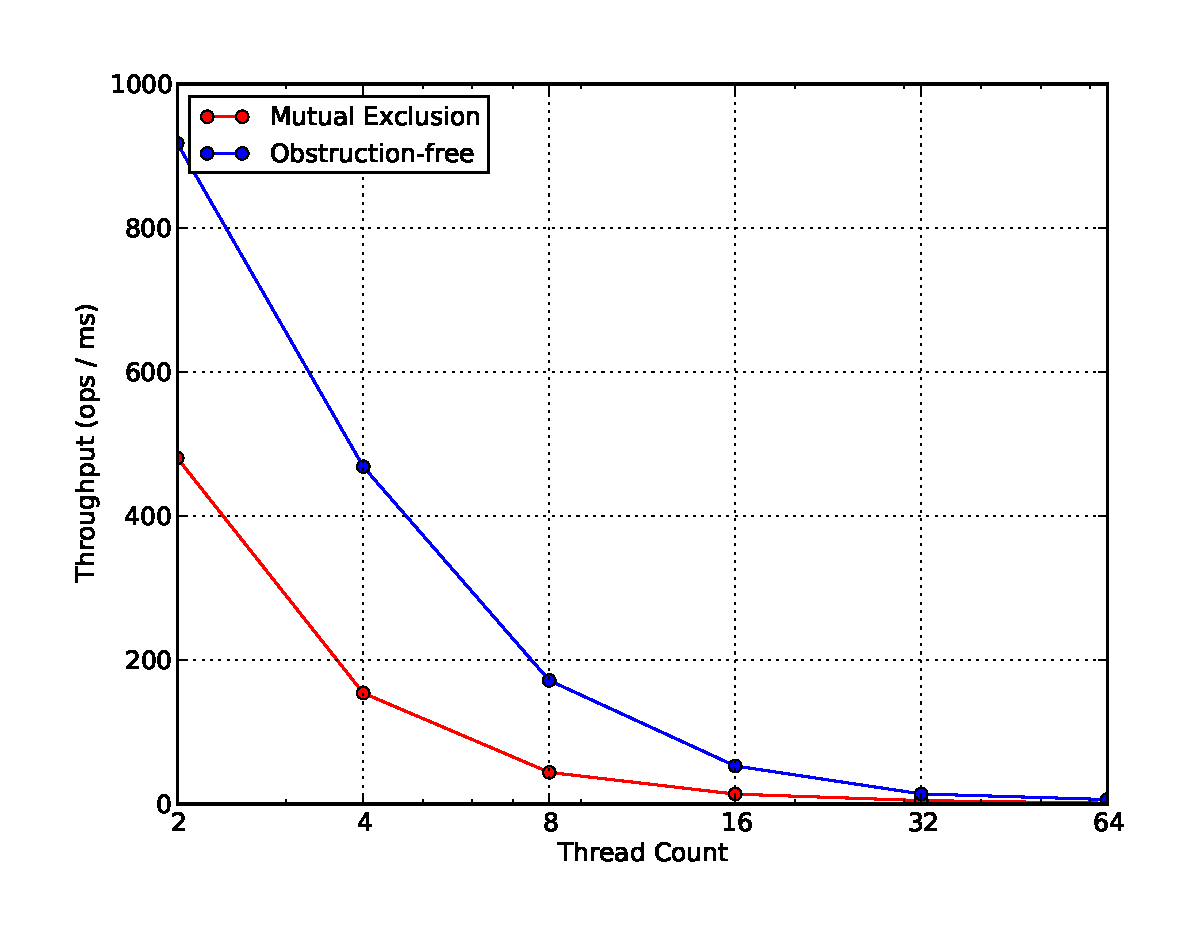
\includegraphics[width=0.5\textwidth]{herlihy/exp/throughput_push.pdf}
            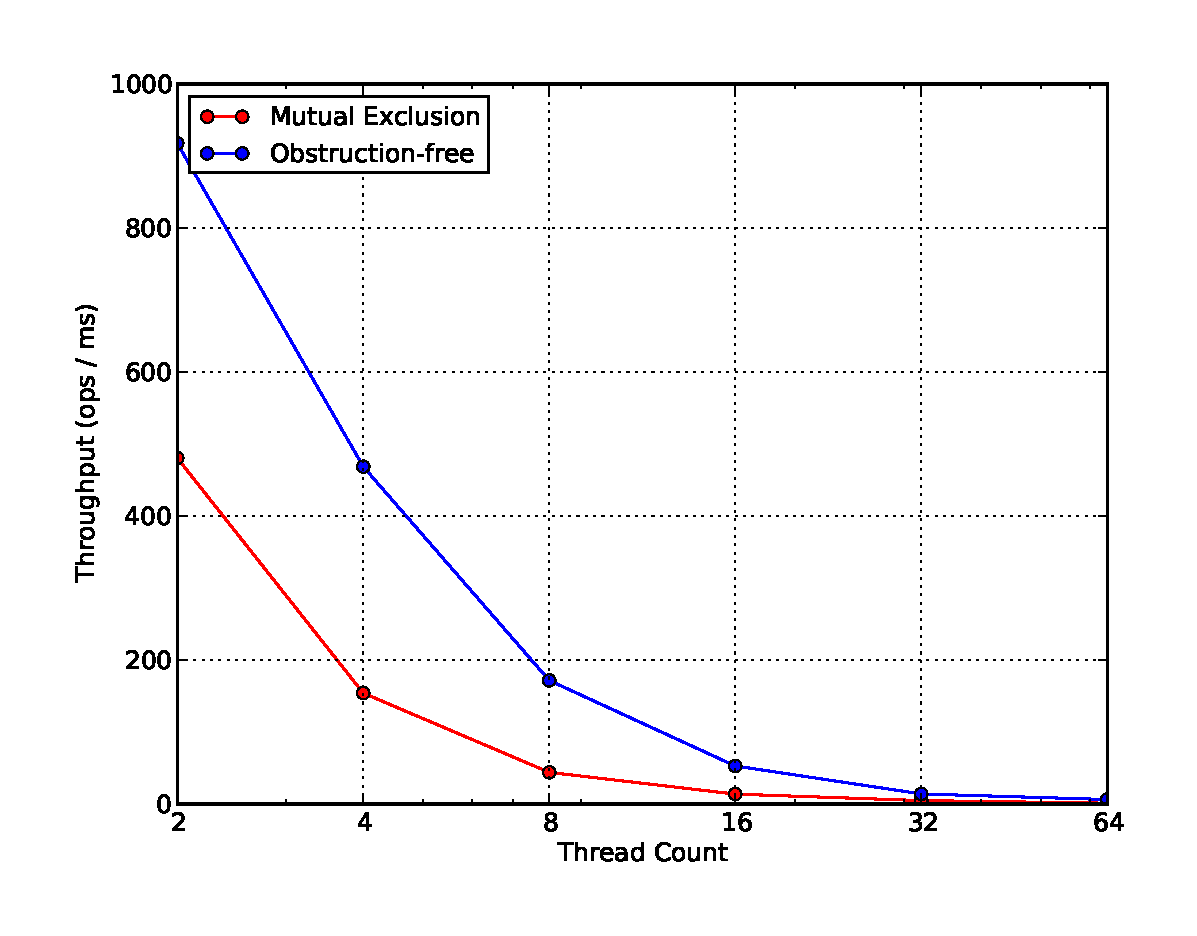
\includegraphics[width=0.5\textwidth]{herlihy/exp/throughput_pop.pdf}
            \caption{Throughput of my bounded double-ended queue with a naive test-and-set lock, compared with the throughput of my nonblocking double-ended queue. Left: push operations, right: pop operations.}
            \label{figure::deque-plot}
        \end{figure}

        In a future edition of this paper, I hope to have similar results for the unbounded deque, as well as some comparisons between space utilization in a large bounded deque vs. an unbounded deque with small buffers.

        \begin{figure}[t!]
            \footnotesize\begin{verbatim}
node = { void *val, int ctr };
hint = { node *nodes, int index };
deque = { hint left, hint right };

rightpush(v) // v is not RN or LN
     while (true) {
         k := oracle(right); // find index of leftmost RN
         prev := k.nodes[k.index - 1]; // read (supposed) rightmost non-RN value
         cur := k.nodes[k.index]; // read (supposed) leftmost RN value
         if (prev.val != RN and cur.val = RN) { // oracle is right
             if(k.index == SIZE - 1) { // need more space
                 buffer = new node[SIZE]
                 buffer[0].val = k.nodes
                 buffer[1].val = v
                 if CAS(&k.nodes[k.index - 1], prev, <prev.val, prev.ctr + 1>)
                     if CAS(&k.nodes[k.index], cur, <buffer, cur.ctr + 1>)
                         update_hints(right, buffer, k.index + 3)
                         return "ok"
             } else {
                 if CAS(&A[k-1],prev,<prev.val,prev.ctr+1>) // try to bump up prev.ctr
                     if CAS(&A[k],cur,<v,cur.ctr+1>) // try to push new value
                         update_hints(right, k.nodes, k.index + 1)
                         return "ok"; // it worked!
             } // end if (prev.val != RN and cur.val = RN)
         }
     } // end while
rightpop()
     while (true) { // keep trying till return val or empty
         k := oracle(right); // find index of leftmost RN
         cur := k.nodes[k.index - 1]; // read (supposed) value to be popped
         next := k.nodes[k.index]; // read (supposed) leftmost RN
         if (cur.val != RN and next.val = RN) { // oracle is right
             if(k.index - 1 == 0) { // need to transfer to next buffer
                 next_left = k.nodes[k.index - 1].val
                 left_cur = next_left[k.index - 3]
                 if(left_cur.val == LN && next_left[k.index - 3] = left_cur)
                     return empty
                 if CAS(&k.nodes[k.index], next, <next.val, next.ctr + 1>)
                     if CAS(&next_left[k.index - 3], left_cur, <left_cur.val, left_cur.ctr + 1>)
                         update_hints(right, k.nodes, k.index - 3)
                         return left_cur.val
             } else {
                 if (cur.val = LN and k.nodes[k,index - 1] = cur)"; // adjacent LN and RN
                     return "empty
                 if CAS(&k.nodes[k.index], next, <RN, next.ctr + 1>) // try to bump up next.ctr
                     if CAS(&k.nodes[k.index - 1], cur, <RN, cur.ctr + 1>) // try to remove value
                         update_hints(right, k.nodes, k.index - 1)
                         return cur.val // it worked; return removed value
             }
         } // end if (cur.val != RN and next.val = RN)
     } // end while
            \end{verbatim}
            \caption{Pseudo-code of a novel unbounded deque. Left operations are completely symmetrical with right operations.}
            \label{code::bounded}
        \end{figure}

    \newpage
    \bibliographystyle{plain}
    \bibliography{citations}
\end{document}